\chapter{Methodology Overview}
\label{sec:methodology}

As the endeavor of this thesis was the merger and enhancement of various aspects of the LORNA project, the complexity lied rather in the understanding of the existing work and the interfaces thereof as opposed to the challenging methodology pursued in the novel contributions. Therefore, the implementation aspect of this work carries more weight than the theoretical decision-making associated with it.

The autonomy framework\citep{Autonomy} allows us to fly independent missions at cruise altitude of 100+ m. The structure from motion approach captures 3D information during traversal as its adaptive baseline allows it to perceive high quality depth information also at such high altitudes. This information can be used by LSD in order to detect landing sites during mission. 

At low altitudes SFM works as well but surrounded with obstacles, the need for lateral motion poses significant risk. This is because a local state estimator is by nature prone to accumulate an estimation error. In this thesis I present a stereo camera implementation to remedy these shortcomings.

% This is because the drone does not retain any hazard information past the knowledge of detected landing sites and terrain knowledge from either HiRISE, Ingenuity or the rover which is implicitly used for the mission creation. Therefore, it could be said that the drone flies blindly with respect to obstacles. 

\section{Stereo Camera}

The implementation of the stereo camera sensor itself is very straightforward as simply duplicating an existing camera, offsetting it an adequate distance to resemble the real model and settings the parameters to equal the hardware results in the desired outcome.

Processing this information is different from for the existing SFM node. Therefore, a new depth generation node was put in place. 

The two images and the drone's base link pose are given to the node as input and processed. Using OpenCV's StereoSGBM algorithm, disparity images are created. These are then converted to point clouds using the stereo depth formula and coordinate transforms from the camera to the world frame. Finally, the stereo camera depth nodes outputs the point cloud in the world frame as well as the two camera poses used to create it.

As the stereo camera has a relatively small, fixed baseline. The usage domain is restricted to low altitudes. The residual part of a mission is still flown using SFM. To facilitate the switch between these two depth sources, the laser range finder sensor was used.

\subsection{Stereo Camera Advantages}

The specific advantage of a stereo camera implementation when compared to SFM can be summarized in the following points:

\begin{itemize}
    \item No necessity of lateral motion
    \item Hardware depth perception
    \item DEM conversion
    \item Efficiency
\end{itemize}

\subsubsection{Lateral Motion}

As already mentioned above the need for lateral motion in itself is an undesirable necessity for a rotorcraft in unknown terrain. 

In this setup the structure from motion approach is based on a key frame buffer which needs to be filled with image-pose pairs at different horizontal positions in order to start acquiring depth information. The current setting in the implementation \citet{SFM} uses 6 key frames. Therefore, for a single point cloud it is necessary to move laterally 6 times in order to start perceiving depth. Following the depth error formula from a stereo disparity image (\ref{eq:SFM_depth_error}) and assuming an altitude of 2.5 m above ground with a focal length of 256 pixels and a disparity error of 0.5 pixels, the necessary baseline in order to keep the depth error below a critical 5 cm is:

\subsubsection{Software vs Hardware Depth Perception}

Structure from Motion, being a software node that relies on camera poses supplied by a state estimator, is by design subject to inaccuracies. A depth node based on a stereo camera on the other hand works with a fixed rigid baseline between the camera views. Thus, for low altitude flights that bear the danger of collision, a more robust hardware approach is preferred.

\subsubsection{DEM Conversion}

As described in \cref{subsubsec:setup:aggregation} the multi-resolution DEM used for depth aggregation in LSD is based on Optimal Mixture of Gaussian cells and thus converges over time. 

According to \cref{subsubsec:setup:haz_seg} the landing sites chosen are likely on terrain with low uncertainty. Because of this landing sites are more likely to be detected and have in general a better quality when the terrain perceived has been viewed.

When a landing site has been selected we need to make sure that the landing site is actually correctly detected and of good quality. For this we would like to (re-)detect landing sites on rather converged terrain. Structure from Motion needs constant lateral motion for this. A stereo camera depth node simply hovers in place for any given amount of time.

\subsubsection{Efficiency}

All in all the stereo camera setup allows us to perceive a landing site at course altitude and after having traversed horizontally to that location, we can simply descend to a stereo camera friendly altitude for the verification. Compared to repeated lateral coverage of the area in question this is a huge increase in efficiency.

Looking in depth at the stereo alternative of depth generation, we can first analyze the theoretical threshold of this system.

\section{Theoretical Analysis}

When it comes to depth perception the obvious drawback of a stereo camera is its limited baseline. It only perceives depth accurately for objects within a certain proximity to the lens. 

Assuming a perfectly calibrated and rectified camera there is still always an inaccuracy in the depth estimation arising from the disparity error.

From a given disparity estimate the depth error is derived as follows:

\begin{equation}\label{eq:depth_from_disp}
    z = \frac{f \cdot b}{d}
\end{equation}

Where b is the z is the depth estimate, b is the baseline, f is the focal length and d is the disparity value.

Taking the derivative of z w.r.t. d we get

\begin{equation}
    \frac{\partial z}{\partial d} = - \frac{f  \cdot b}{z^2}
\end{equation}

And substituting (\cref{eq:depth_from_disp}) we get:

\begin{equation}
    {\partial z} = \frac{z^2}{f  \cdot b}\partial d
\end{equation}

Where the sign was left away as for our application there lies equal danger in a point being perceived too close and too far away.

For the maximum altitude given a maximum allowable depth error this yields:

\begin{equation}
    z_{\text{max}} = \sqrt{\frac{\Delta z_{\text{max}} \cdot b \cdot f}{\Delta d}}
\end{equation}

Where $\Delta z$ is the depth error and $\Delta d$ the disparity error.

The stereo camera mounted on the drone in JPL's aerial vehicle lab had a baseline of about 10 cm and a focal length of 256.

With these properties and estimating a subpixel-precision disparity error of 0.5 pixels the depth error at varying altitudes looks as follows:

\begin{figure}
    \centering
    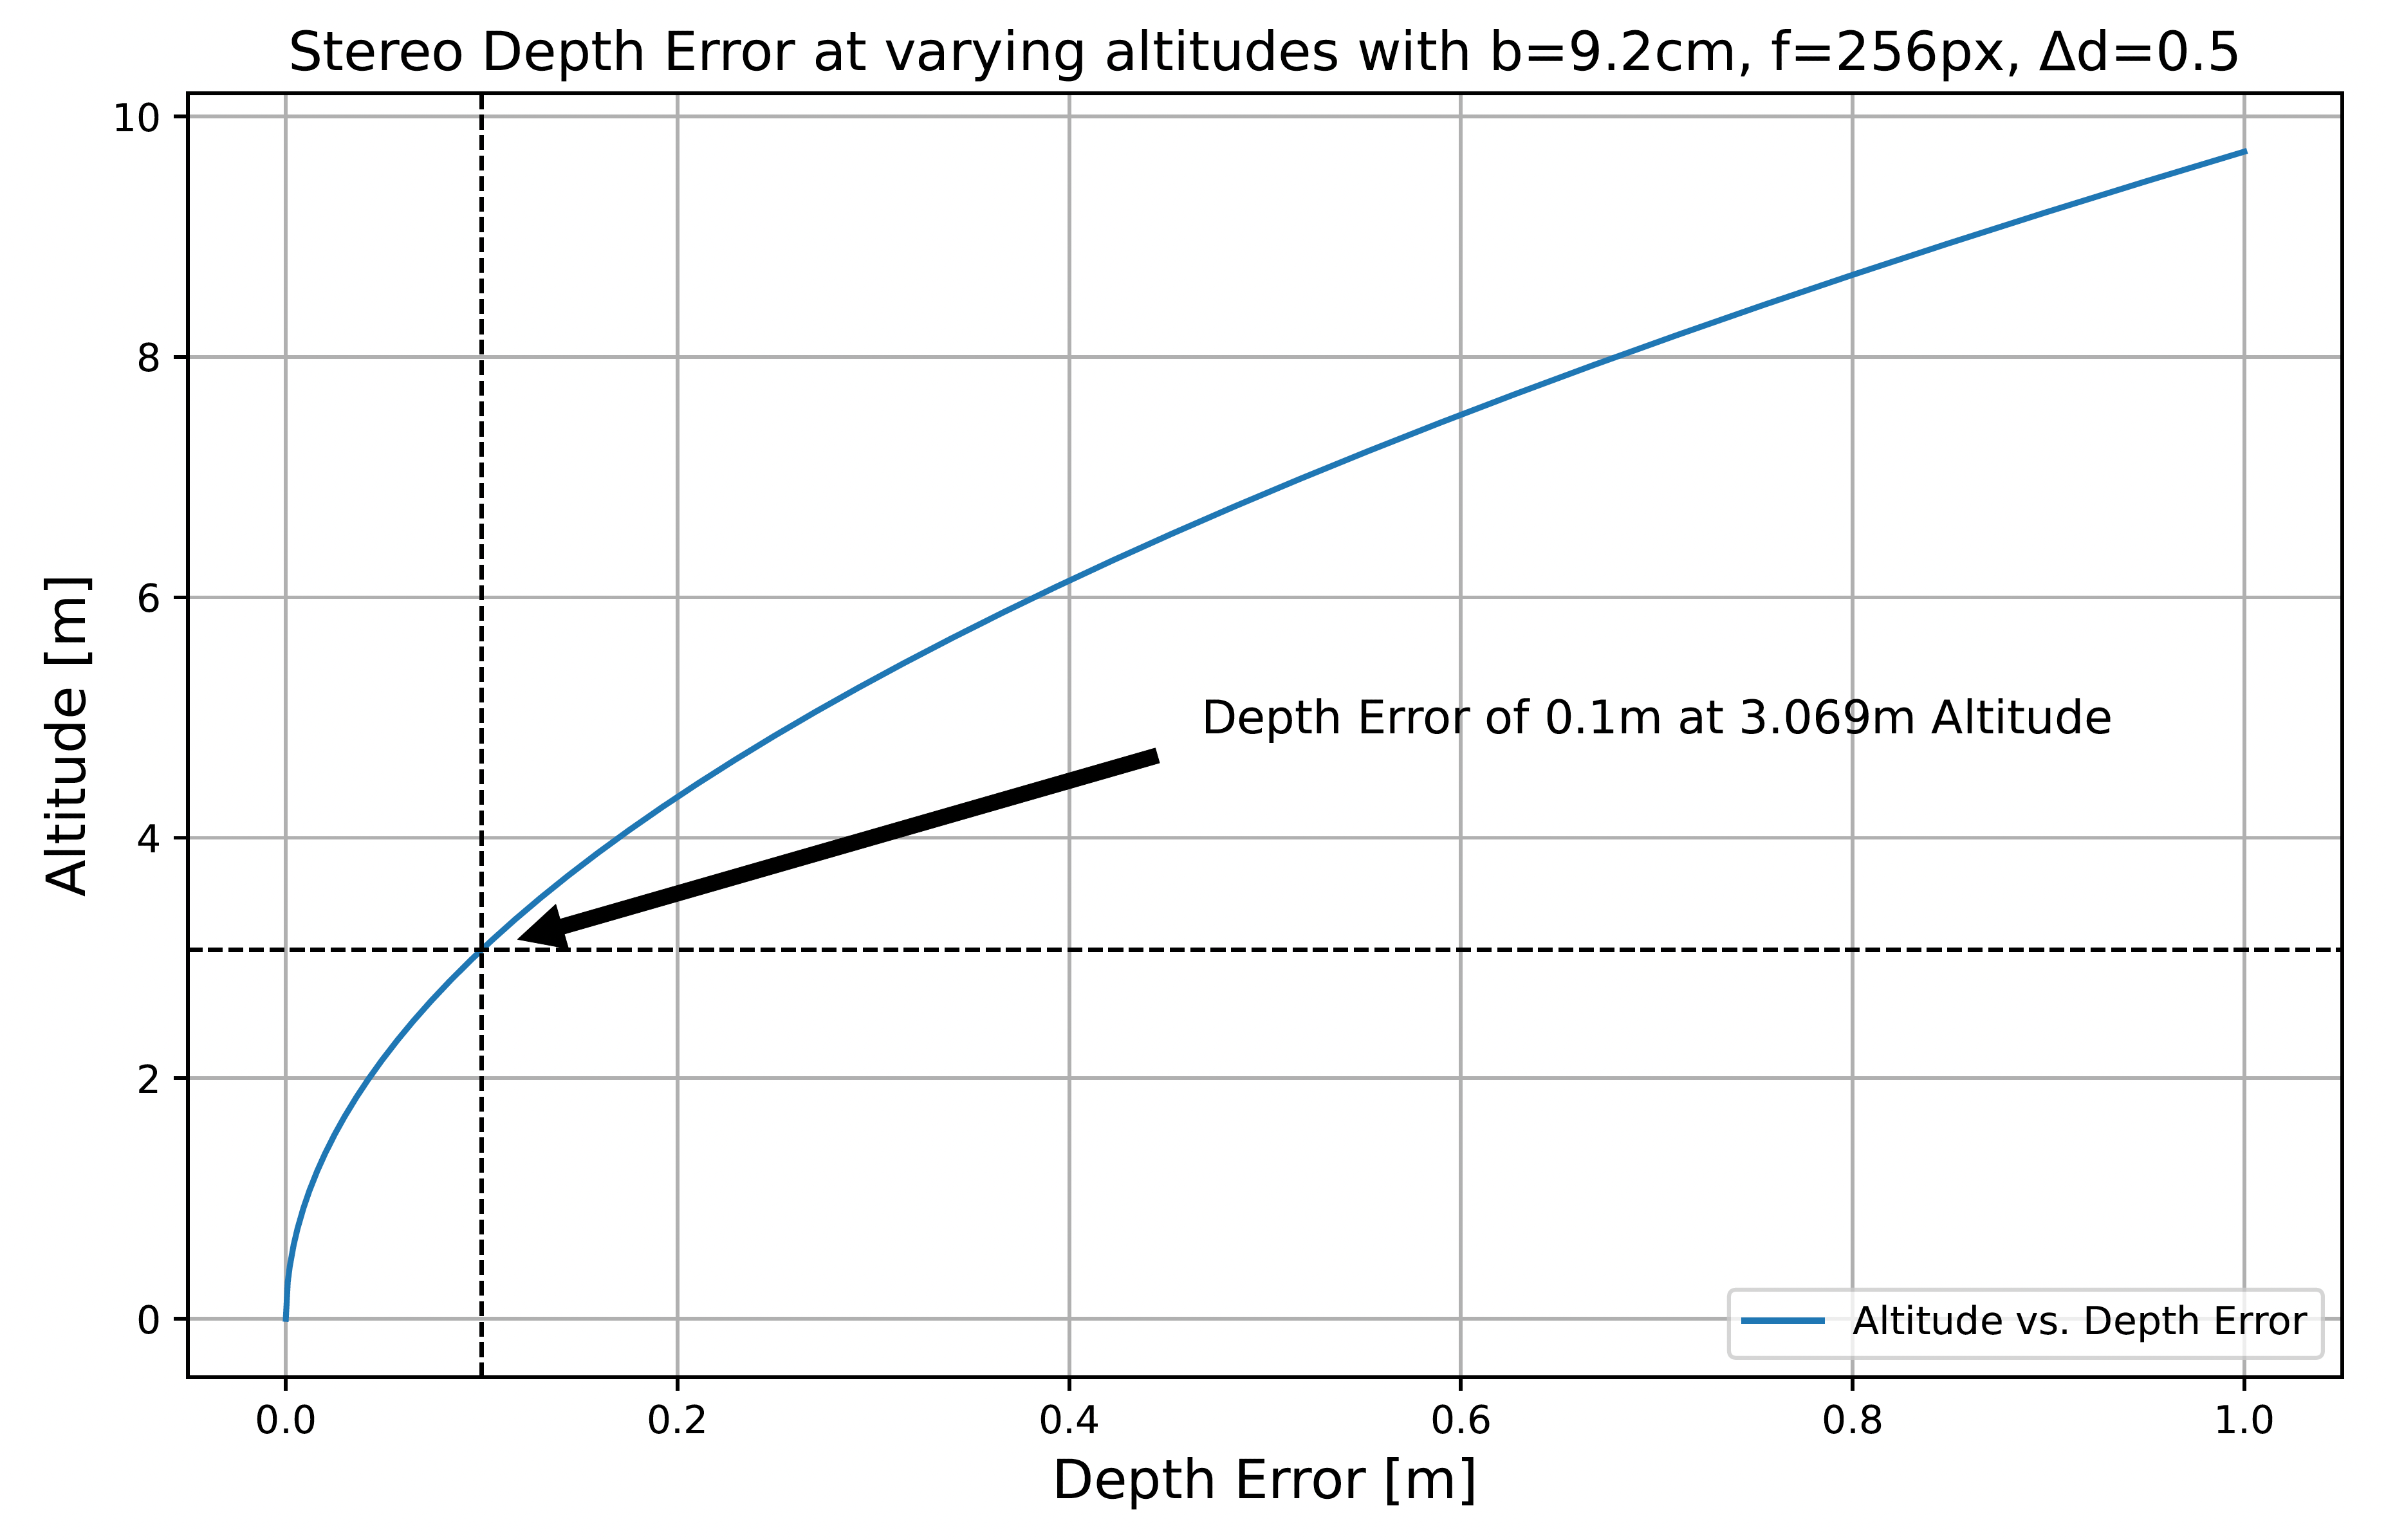
\includegraphics[scale=0.19]{images/preparation/stereo_limit.png}
    \label{fig:stereo_limit}
\end{figure}

Let's assume we allow a maximum depth error of 10 cm. Considering this constraint we can fly at a maximum altitude of about 3 m as indicated in \cref{fig:stereo_limit}.

This limitation has to be kept in mind. However, it is neither too surprising nor is it too restrictive as the stereo camera is simply a depth alternative for low altitude flight maneuvers. In the context of an entire science mission it is almost exclusively used for landing site verification purposes.


\section{Ground Truth Depth}

For evaluation purposes as well as proof of concept aspirations, a ground truth is required. The simulation already supplied the ground truth pose of the drone's base link through the ROS bridges. When applying the static camera transform to it, this yielded the ground truth camera pose. Using Gazebo's depth camera sensor\footnote[1]{As there was a bug in Gazebo's source code, the depth camera couldn't be used out of the box. More on this in \cref{chapter:appendix:gz_depth_camera}.}, a ground truth point cloud could be created.

The depth camera creates the image using traced rays which fill a pixel with the center most range value that a ray detected.

As expected, the ground truth point clouds yielded very clean and easily interpretable LSD DEMs:

\begin{figure}[ht]
\centering
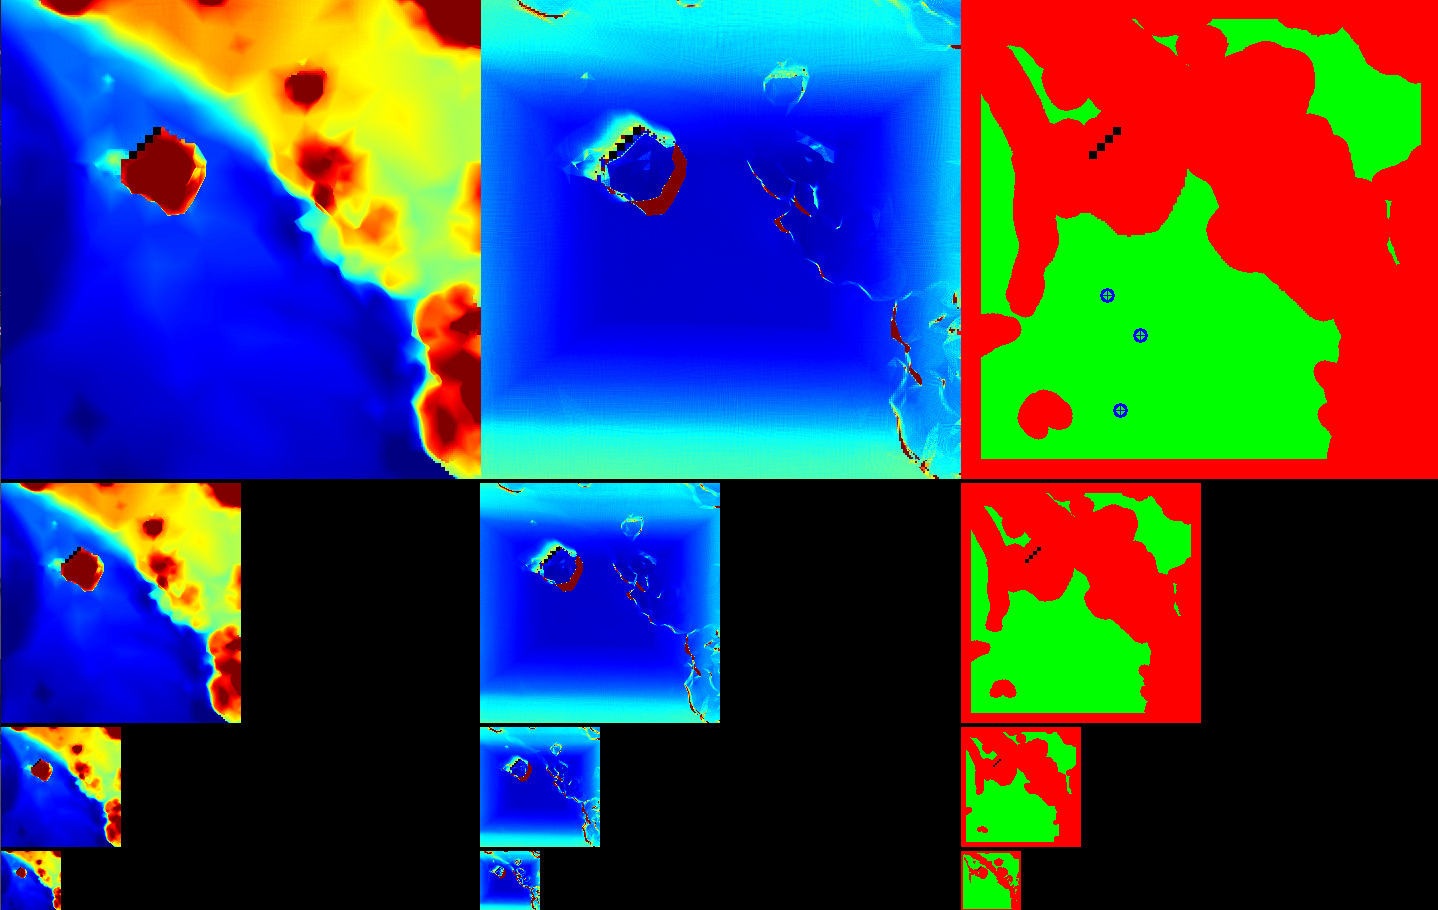
\includegraphics[scale=0.25]{images/methodology/lsd_debug_image.png}
\caption{LSD debug image using a GT point cloud}
\label{fig:gt_lsd_debug}
\end{figure}

\begin{figure}[ht]
\centering
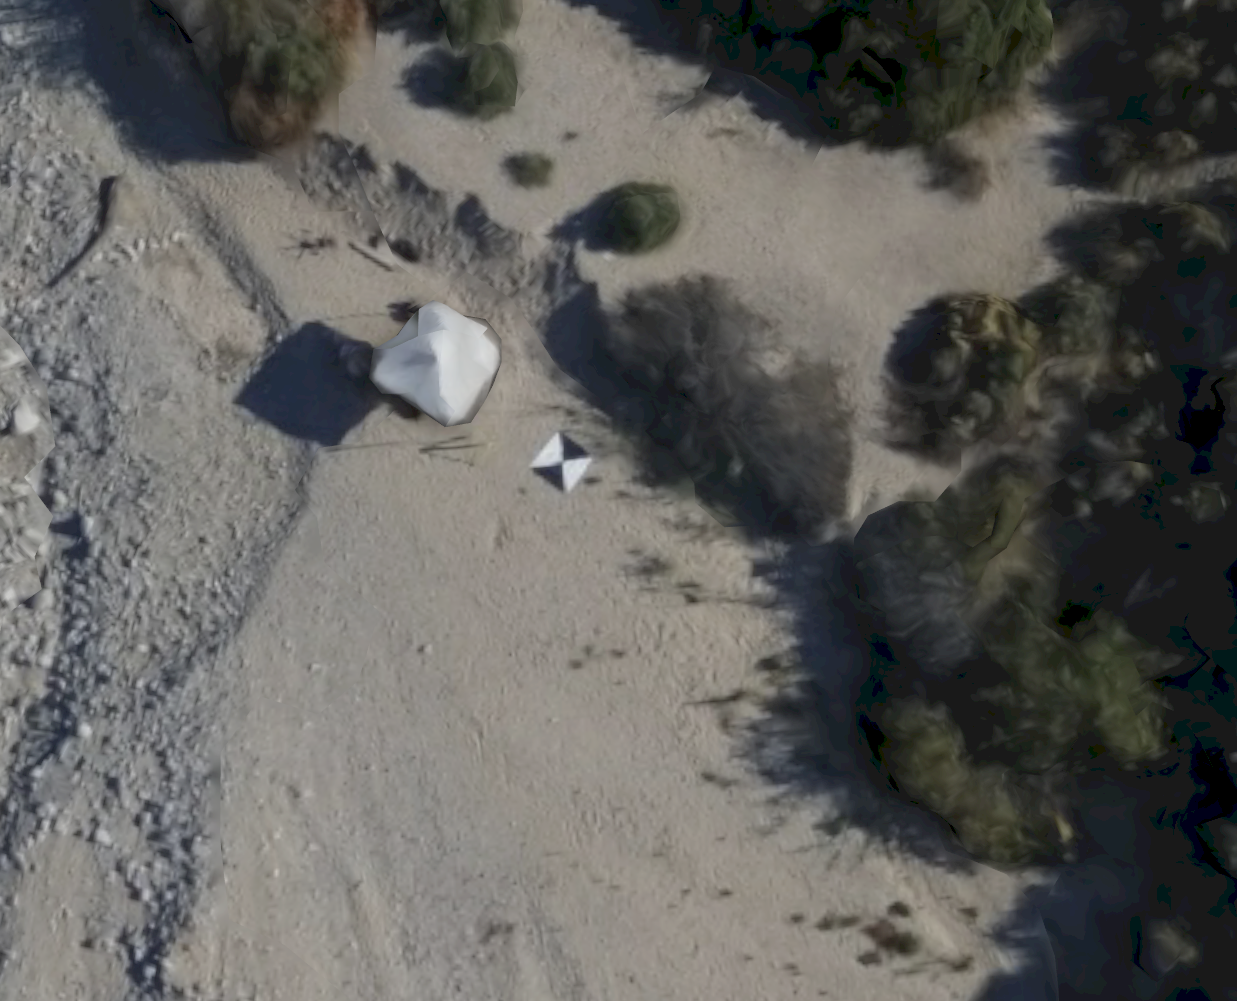
\includegraphics[scale=0.25]{images/methodology/lsd_debug_reference.png}
\caption{LSD debug image simulation terrain reference}
\label{fig:gt_lsd_debug_reference}
\end{figure}

\subsection{Comparability to SFM}

This is sufficient for a qualitative analysis of the stereo depth node. However, to use the ground truth as an alternative for SFM, one has to make sure that the GT quality is not too good. For instance, SFM, like the stereo camera depth, has a depth error associated with its point cloud creation. At high altitudes this can lead to the neglect of small (but for the drone threatening) rocks. So, in order to test the autonomous landing pipeline with ground truth, I had to make sure that small rocks of about 10 cm diameter were not seen by the GT at a cruise altitude of 100 m.

For this, the following test was designed.

On a flat textured plane, three cylinders of different sizes were placed. On each cylinder a small rock of 10 cm diameter was placed. The drone was then flown over the test setup to detect the scene once with SFM and once using the GT depth. The goal was to find out, whether the ground truth depth quality would have to be artificially decreased, using Gaussian or median filtering for instance, in order to make it more comparable to SFM.

\begin{figure}[ht]
\centering
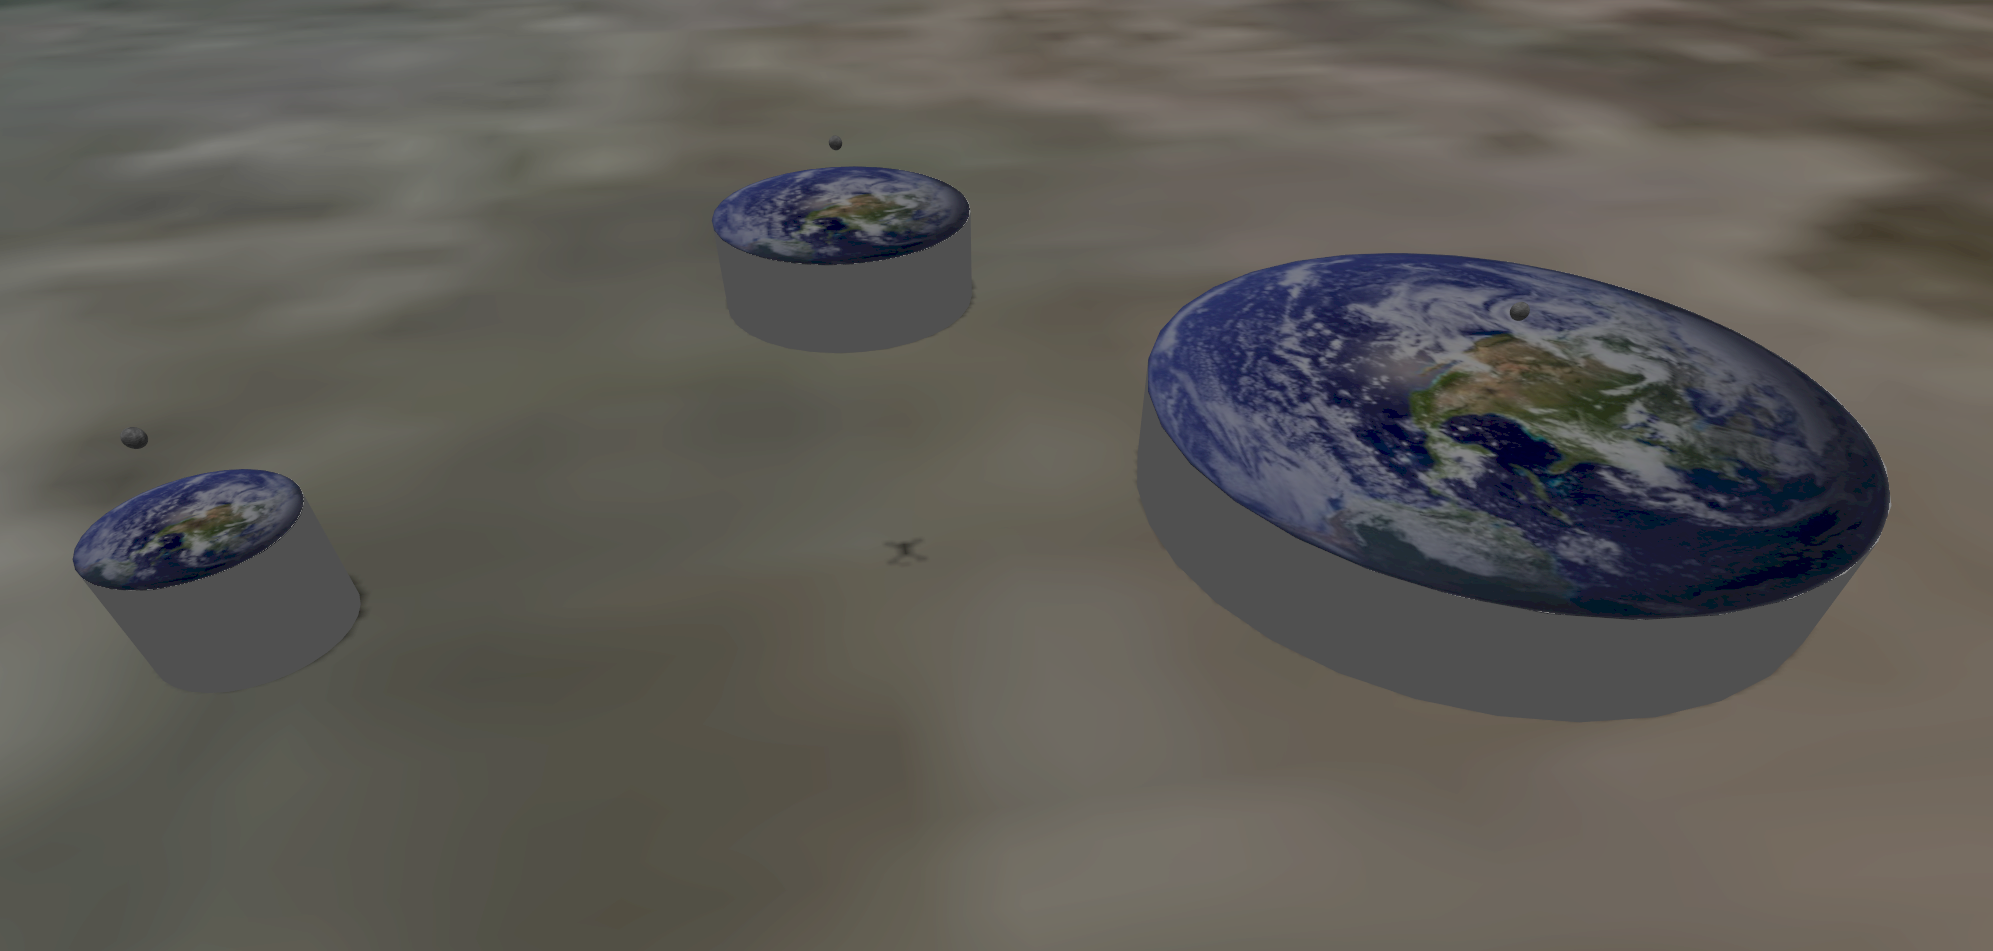
\includegraphics[scale=0.18]{images/methodology/Test.png}
\caption{GT test setup: Rocks of 10 cm diameter where placed on platforms of different sizes to be detected by both the ground truth and SFM}
\label{fig:gt_test_setup}
\end{figure}

\begin{figure}[ht]
\centering
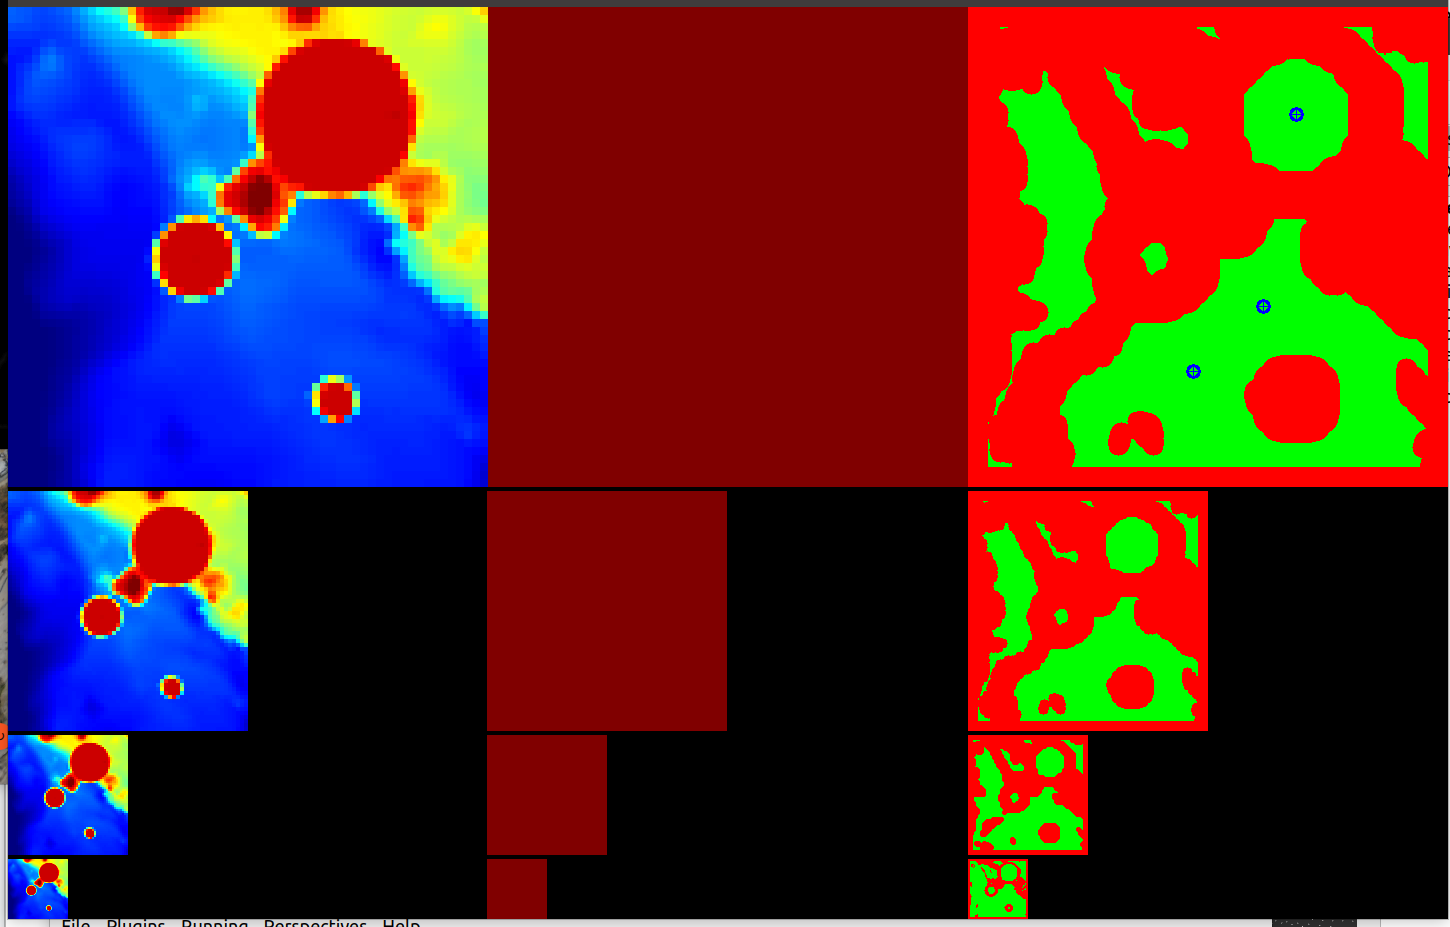
\includegraphics[scale=0.14]{images/methodology/GT.png}
\caption{Ground truth result of the GT test}
\label{fig:gt_test_gt}
\end{figure}

\begin{figure}[ht]
\centering
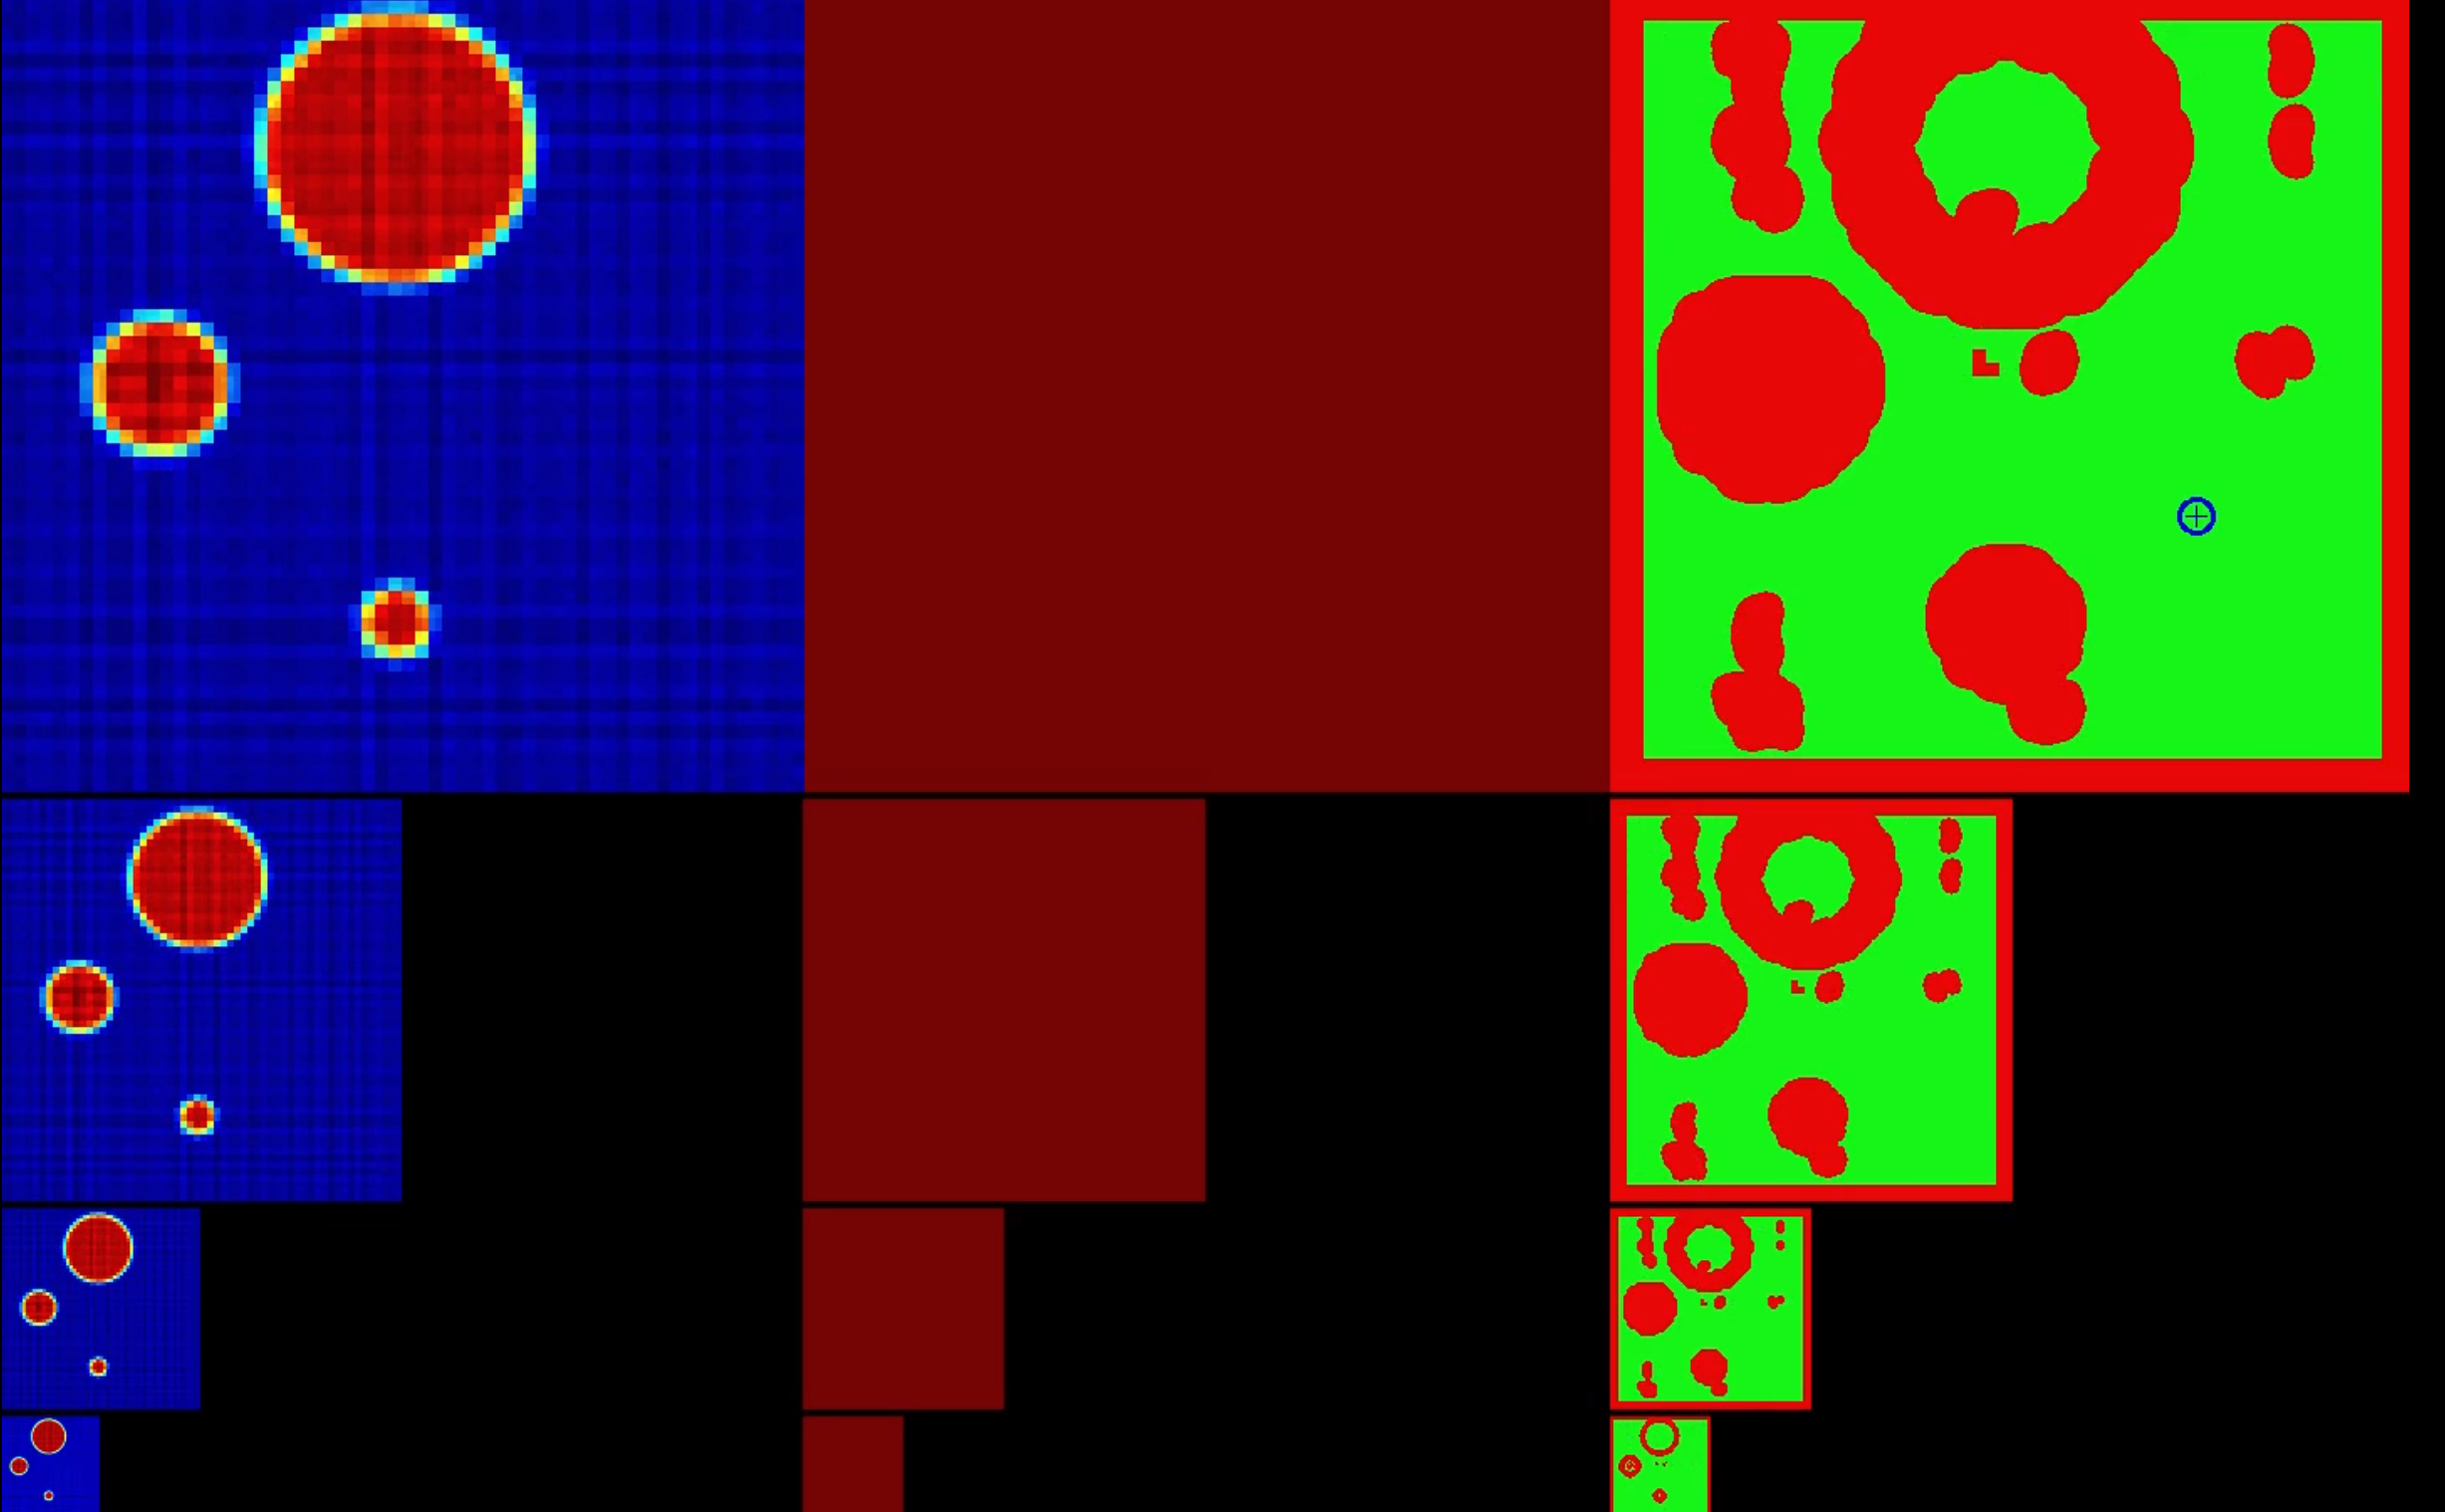
\includegraphics[scale=0.14]{images/methodology/SFM.png}
\caption{SFM result of the GT test}
\label{fig:gt_test_sfm}
\end{figure} %TODO redo this test and get better images

Looking at \cref{fig:gt_test_gt} and \cref{fig:gt_test_sfm}, one can see, that, though the SFM quality is visibly worse, neither SFM nor GT detected the small rocks on the platforms. This can be seen because in both Debug images the center of the platforms was considered a landing site even though there was the rock which should definitely prevent the detection of a valid landing site.

Therefore, the ground truth depth could be used for the testing of the autonomous landing pipeline without making a landing site verification step at low altitudes redundant.


\section{Autonomous Landing Procedure}

Having implemented a stereo camera as a low altitude alternative to SFM and after ensuring a correct ground truth comparison, the main contribution of this work could be tackled: Bringing the visual landing site pipeline together with the autonomy framework in order to achieve reliable autonomous landing in unknown terrain.

The approach of the landing pipeline implementation can be split into the following parts:

\begin{itemize}
    \item Landing site detection output

    Prior to this work, LSD only published one single landing site's location. To give the autonomy more information to make adequate decisions and to avoid the stagnation on a single overconfident landing site, LSD is changed to also first, publish three landing sites each iteration and secondly, yield additional characteristics with each output landing site.
    \item Landing site interface of the autonomy

    The autonomy framework is changed to correctly receive and handle incoming landing sites. The incoming candidates are ordered according to a novel landing site heuristic and updated upon being re-detected.
    \item Autonomous landing behavior

    Using the newly expressive landing sites and their handling procedure, the adaptive landing instance is put in place using an existing behavior tree framework within the autonomy. Additional modular action nodes are created and previously existing ones are altered in order to achieve a precise and safe landing procedure.
\end{itemize}

% TODO Write out LSD preparation aka to prepare for lanidng this and this...
\section{Landing Site Handling}\label{subsubsec:LandingSiteHeuristic}

\subsection{LSD Properties}\label{sec:LSproperties}

With the low altitude depth alternative in place, the connection of the autonomy with the landing site detector could be tackled. 

Before this work the output of the landing site detection algorithm was merely the location of a found landing site. However, as described in \cref{subsubsec:setup:haz_seg} the landing site detection algorithms segments hazards based on roughness and slope. Subsequently, it considers the size of a landing site as well as the uncertainty associated with a certain selected location. 

Simply outputting the location of a landing site is therefore a waste of information when so many characteristics are at hand to make an informed selection. 

I decided on the following properties to be the LSD output:

\begin{itemize}
    \item Location
    \item Uncertainty
    \item Roughness
    \item Size
    \item Obstacle Altitude
\end{itemize}
The final landing site detection output is a custom landing site ROS message containing the above-mentioned characteristics of the detected spot.

\textbf{Location}

The location of the landing site in the world frame.
\textbf{Roughness}

The roughness value the exact value already used for the hazard segmentation step in the landing site detection. 

\textbf{Uncertainty}

The uncertainty value is also a product of the landing site detection algorithm. It denotes the averaged uncertainty across the area around a given landing site. The uncertainty of a single map cell denotes the stereo depth error estimates merged over time.

\textbf{Size}

To determine the size of a landing site, the landing site detection algorithm performs a distance transform on the created landing site map in order to find the closest non-landing site for any found landing site. This returns the radius of the largest valid landing circle around a landing site. Calculating the physical value, the metric radius is returned as the size of a landing site.

\textbf{Obstacle Altitude}\label{subsec:obstacle_altitude}

The obstacle altitude was newly introduced in this work. It defines the current highest point of the aggregated DEM's highest resolution layer. As no actual object detection is performed and no hazard information is retained in this visual pipeline, this value serves the autonomy as an indication of the obstacles heights to avoid in the vicinity of a certain landing site. More on this in \cref{subsubsec:LandingSiteHeuristic}.

\subsection{Landing Site Heuristic}

The autonomy processes the in \cref{sec:LSproperties} listed values in order to arrive at the following final landing site properties:

\begin{itemize}
    \item Current Distance to Drone
    \item Roughness
    \item Uncertainty
    \item Size
    \item Verification Altitude
\end{itemize}

The final heuristic defining the quality of a landing site is in fact a square loss function:

\begin{equation}
    L_{LS} = w_{dist}L_{dist} + w_{rough}L_{rough} + w_{var}L_{var} + w_{size}L_{size} + w_{verAlt}L_{verAlt}
    \label{eq:loss_fct}
\end{equation}

\textbf{Current Distance to Drone - $L_{dist}$}
Well likely the single most important characteristic of a landing site\footnote[1]{Each received landing site has already undergone a threshold filtering regarding slope and roughness.}. Each iteration the current distance to the drone's position is calculated for each retained landing site. The distance is then normalized by dividing it by the cruise altitude which is 100 m. In practice there were easily enough landing sites found while moving to allow landing sites to fall off when being farther away than 100 m.

\textbf{Roughness - $L_{rough}$}
%TODO

The roughness property is the unaltered roughness value received from LSD. It is already normalized and enters the loss function as it is. 

\textbf{Uncertainty - $L_{var}$}

The same holds for the uncertainty. It is already normalized by design and enters the loss function unaltered.

\textbf{Size - $L_{size}$}

Analogous to the roughness and uncertainty properties the size comes from the landing site detection directly. However, unlike the two preceding properties it is not normalized but simply denotes the metric radius of the largest circle of valid landing area that can be fit around a given landing site. This is achieved in LSD by performing a distance transform on the created landing site image.

In order to normalize this value the maximum landing site size is retained and each landing site's size is divided by it in order to achieve normalized size information.

Also, as can be seen in \cref{eq:loss_fct}, the size contribution enters the loss function with a negative sign. This is due to the fact that compared to all other characteristics, the size defines a property that we would like to maximize.

\textbf{Verification Altitude - $L_{verAlt}$}\label{subsubsec:ver_alt}

A site's verification altitude is the smallest vertical distance between the drone and the landing site at which that site was (re-) detected. 

The verification altitude is a useful property because of numerous reasons.
\begin{itemize}
    \item Further Indication of Certainty

    First, similar to the uncertainty metric the verification altitude indicates how certain we can be about a detected landing site as spots detected at lower flight altitudes are more likely correct due to the reduced depth error. Even though it might seem overlapping with the uncertainty property in this regard, these two characteristics are quite complementary as the uncertainty takes OMG convergence and camera specifics into consideration while the verification altitude is a purely location based metric.
    \item Landing Site Property Updates

    As the verification altitude yields a simple and good estimation of the trustworthiness of an incoming landing site, it can be used as a flag to know, when a landing site's properties should be updated. When a landing site is re-detected with a verification altitude lower than the previously stored one, the algorithm trusts it more and alters the previously stored properties to the new ones received.
    \item Verification

    Continuously updating the verification altitude upon re-detection allows us to determine the lowest altitude, at which a landing site was re-detected. This information can be used to verify that a given site was considered a valid landing spot even at low altitudes. 
\end{itemize}

\subsection{Landing Site Manager}

Prior to this thesis, the landing site manager received artificially generated landing sites from a dummy landing site node. In this work the LSM was connected to the actual landing site detection output. 

% Added re-detection, verification and banning

\subsection{Implementation}

With the interface and the input fixed, the actual implementation could be tackled. This is explained in detail in \cref{chapter:autonomous_landing_procedure}.
